\chapter{Requirements Analysis}
\section{Top Level Requirements:}
\begin{enumerate}
   
\item{\bf Gather News Feed: }
 The application must gather news articles around the world for the users. This is planned to be accomplished through querying News Api which has categories and country fields and updating database with sample data to make it reliable for application.
 \item{\bf Personalization: }
 The application is mainly focused on delivering news based on user personalization aspects. For achieving this requirement, the application targets two main concepts\cite{authentic.} which are Contextual and Behavioral Personalization. 
 Application is expected to develop Contextual personalization by building location-specific news and user-preferred categories news data in their personal feed.
 Also, in terms of behavioral the application is targeted to achieve personalization based on user interactions which includes the likes, save or add to favorites.
 Additionally, the application has to develop a way to recommend news articles to the users for which Mahout Recommendation system is considered for analysis.
 
 \item{\bf Visualization: }
 The application is aimed to have more interactive views for the user where the amcharts map for the location filter and charts for projecting user category-specific interest rate are desired to be achieved.

\end{enumerate}
 \section{Detailed Requirements}
 
 \textbf{ \large Essential Requirements}
 \begin{enumerate}
 \item{\bf User Authentication:}
 The user registration should be feasible and the registered users should be able to login with a valid token.
 \item{\bf News Feed:}
 The application has to gather news from a well-defined api which has all essential fields of our news model.
 \item{\bf Database:}
 The news api has to be queried and updated to database with sample data for reliability of application especially during presentation to avoid any issues.
 \item{ \bf Personalization:}
 The main feature of personalization to be well-designed and also updating for changing user's interests.
 \end{enumerate}
 \textbf{ \large Recommended Requirements}
 \begin{enumerate}
 \item{\bf User Charts:}
 The application should be designed to project user category chart which shows percentage of interests for various news categories.
\item {\bf User Profile:} There should have options for users to view their profile anytime in the application view.
\item{\bf Visualization:}
The application has to have a globe view to help users to choose any country to view the location-specific data and filter through categories if applicable.
\end{enumerate}
 \textbf{ \large Optional Requirements:}
 \begin{enumerate}
 \item{\bf Category Newsfeed:}
 The application has to load separate category data into various view for easy access.
 \item{\bf Saved/ Favorite feed:} The application could have the option to show users saved and favorite feeds for them to revisit anytime.
 \item {\bf Update Profile: } The option to update the profile details for the users could be better.
\item{\bf Recommendation System:} The application is desired to have the recommendation of news articles for users based on their interest pattern.
\end{enumerate}

\section{ Technical Specification}
\begin{center}
    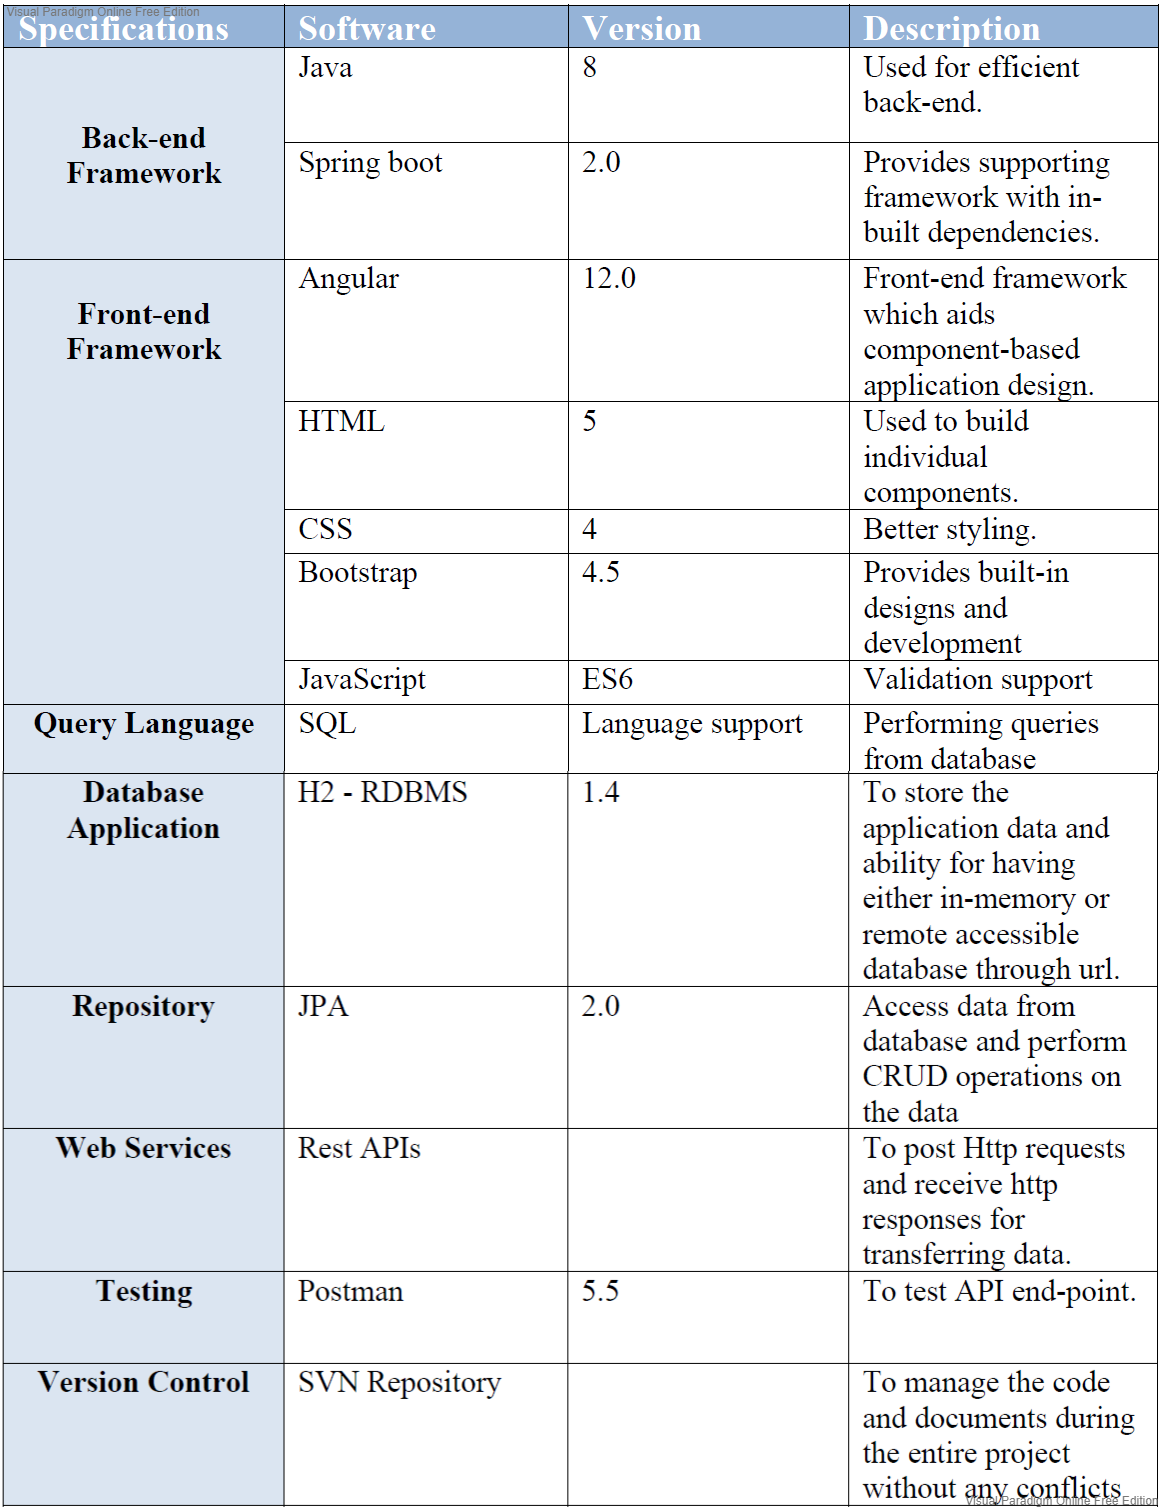
\includegraphics[scale=0.3]{images/techspecs.png}
    
\end{center}
